plate \graphicspath{{chapters/6.Chapter_4/figures/}}

\begin{savequote}[75mm]
In biology, nothing is clear, everything is too complicated, everything is a mess, 
and just when you think you understand something, you peel off a layer and find 
deeper complications beneath. Nature is anything but simple.
	\qauthor{- Richard Preston: The Hot Zone}
\end{savequote}

\chapter{RNAi in \textit{P. bursaria}}

\section{Introduction}

\subsection{RNAi}

Post-transcriptional gene silencing (PTGS) is a highly useful experimental technique
in reverse genetic analysis of a given gene.  
The most widely used PTGS method is that of RNA-mediated inteference (RNAi)
of gene expression. 
RNAi \citep{Fire1998} is a powerful experimental technique which is widely used 
in the study of model eukaryotic organisms \citep{Morf2013,Batista2011,Matthew2004,Ketting2011,Chang2012}.

RNAi covers a set of evolutionarily conserved mechanisms across the eukaryotes 
with numerous mechanisms in which the expression of particular transcripts
is regulated via several classes of transcribed small non-coding RNA (ncRNA)
such as short-intefering (siRNA), micro (miRNA) and Piwi-interacting (piRNAs) \citep{Carthew2009}.

These systems likely originated as a form of defence against
viruses and transposons \citep{Waterhouse2001,Buchon2006}
and were present in some form in the last universal eukaryotic
ancestor (LECA) \citep{Cerutti2006,Shabalina2008}.  Many eukaryotes
utilise these small RNA-mediated gene silencing pathways
in the regulation of their own cell expression patterns \citep{Wu2008}.
Despite its ancestral nature there has been considerable diversification
of both this process, its function and mechanism \citep{Ketting2011}.
Indeed, even with the same organism, different points of the life cycle
may use different RNAi systems \citep{Flemr2013}.


Generally RNAi pathways involve the generation of 21-28nt short RNAs
from some form of RNA precursor such as dsRNA (or ssRNA)
via the function of the RNAase III Dicer \citep{Bernstein2001} or related proteins.
These short RNAs are then bound by Argonaute proteins which act alone or as part
of a complex to silence the expression of sequences homologous to the siRNA \citep{Ketting2011}.
This silencing isn't just limited to the post-transcriptional endonucleocytic degradation of 
mRNA transcripts but can also involve transcriptional inhibiton and
DNA elimination \citep{Marker2014}.
The one unifying element of all discovered RNAi pathways is that
of the central role argonaute (AGO) proteins play \citep{Ketting2011}.
They are formed of two subclasses: the Ago and Piwi subfamilies \citep{Peters2007}
with a range of functions and complex-forming behaviours
\citep{Ender2010}.
The magnitude of the silencing response is occasionally amplified by the generation
of more copies of the trigger dsRNA by RNA-dependent RNA polyermases (RdRPs) \citep{Arp2007}.
On the other hand RdRPs can also sometimes directly generate the siRNAs \citep{Aoki2007,Ketting2011}.
Interestingly, the last universal eukaryotic ancestor (LECA) likely contained 
at least one Ago and Piwi family Argonaute protein, a Dicer and an RdRP \citep{Cerutti2006}.

The two main systems are the siRNA and miRNA based systems.  They are differentiated
by miRNAs being encoded by dedicated genes and displaying partial
complementarity to their targets whereas siRNAs are generated from exogenous
dsRNAs (i.e. environmental dsRNA from viral infection or phagocytosed bacteria \citep{Whangbo2008})
or transgenes and involve full or near full complementarity \citep{Shabalina2008}
However, there are also piRNA systems involved in germline based transposon silencing \citep{Iwasaki2015}.
An important ciliate specific system is that of scan RNAs (scnRNAs) which 
are involved in the elimination of internal eliminated sequences (IESs) during
macronuclear (MAC) regeneration \citep{Mochizuki2004,Chalker2013}.


Experimentally, the existence and function of these systems
permits a researcher to introduce dsRNA homologous to an RNA transcript of interest
and trigger targeted cell-wide RNAi of that transcript.
Unforunately, there also several problems with RNAi as a general method.
Many organisms lack active RNAi systems, although such systems can occasionally
be induced \citep{Alibu2005}.
On top of this, RNAi requires exact sequences to design precursors.
In order to minimise off-target effects, in which a provided sRNA precursor induces RNAi
in more than just the target transcript, a complete genome and/or transcriptome
is useful in the design stage as off-target hits can be checked. 
Off-target effects  can lead to cryptic
phenotypic outcomes that are then falsely attributed to the initial target.
Another problem is that RNAi does not necessarily induce total silencing
of a given transcript and low-levels of transcription may still occur.
This, conceivably, can be sufficient to maintain the non-knock down phenotype.

\subsection{RNAi in \textit{Paramecium}}

In addition to the scnRNA system mentioned above siRNA
based pathways have been discovered in the two principal
ciliate model organisms: \textit{Tetrahymena thermophila} \citep{Collins2006,Yao2005}
and \textit{Paramecium tetaurelia} \citep{Galvani2001,Galvani2002}. 
There are 2 established methods for inducing RNAi in \textit{Paramecium tetaurelia}:
microinject and transformation of the MAC with high-copy transgenes lacking 3' untranslated
region (UTR) \citep{Galvani2001} and the introduction of dsRNA by either
microinjection or feeding using transformed dsRNA expressing bacteria 
\citep{Galvani2002}.

In the transgene pathway, the 3' truncation to the production of aberrant
sense and antisense transcripts \citep{Galvani2001,Marker2010,Beisson2010b}.
Based on the identified required components (see \cref{tab:marker_components}), 
aberrant transcripts
are processed by a Dicer protein (Dcr1) \citep{Lepere2009} and
an putative RdRP complex formed of an RdRP (Rdr2) and a nucleotidyl
transferase (Cid2) \citep{Marker2014} into 23nt siRNA \citep{Lepere2009}. 
A putatively non-catytic 
RdRP (Rdr3) also plays an undefined role in the generation
of primary (\(1^{\circ}\)) siRNAs from transgene pre-cursors \citep{Marker2010,Marker2014}.
Finally, two Argonaute Piwi proteins (Ptiwi13 and Ptiwi14) \citep{Bouhouche2011} 
are involved in targeting post-transcriptional silencing via mRNA
cleavage \citep{Bouhouche2011,Marker2014}.


Alternatively, the exogenous dsRNA pathway can be induced by either microinjection directly
into the MAC (for a transient 48 hour long silencing) or by continue feeding
with a bacterially experimentally modified to generate dsRNA.
Typically, this involves an \textit{E. coli} 
with an IPTG-inducible T7 polymerase and 
deficiency for RNAse III containing a plasmid with a T7 promoter and sequence
homologous to the target transcript
\citep{Fire1998,Timmons2001,Galvani2002}.
Interestingly, there is some evidence that this pathway also is activated at low
levels by ssRNA from normal food bacteria \citep{Carradec2015}.

\begin{table}
    \centering
    \begin{tabular}{|c|c|c|}
        \hline
        \textbf{Pathway} & \textbf{Component} & \textbf{Function} \\
        \hline
        transgene-induced siRNA & Rdr3 & RdRP \\
                                & Ptiwi14 & Piwi \\
        both pathways           & Rdr2 & RdRP \\
                                & Dcr1 & Dicer \\
                                & Ptiwi13 & Piwi \\
                                & Cid2 & Nucleotidyl transferase \\
        exogenous dsRNA-induced siRNA & Rdr1 & RdRP \\
                                      & Cid1 & Nucleotidyl transferase \\
                                      & Ptiwi12 & Piwi \\
                                      & Ptiwi15 & Piwi \\
                                      & Pds1 & Import of dsRNA? \\
        \hline
    \end{tabular}
    \caption[Summary of RNAi pathway components in \textit{P. tetaurelia}]{Summary
        of the components identified as necessary to the function of both
        primary siRNA RNAi pathways in \textit{P. tetaurelia} as identified
        by forward genetic screens in \citep{Marker2014}}
    \label{tab:marker_components}
\end{table}


Again, based on the components that have been identified as necessary
for this exogenous dsRNA pathway to function (see \cref{tab:marker_components}).  
RNA precursors are processed
by Dcr1 \citep{Lepere2009}, and then two hypothetical RdRC (Cid1-Rdr1, Cid2-Rdr2)
\citep{Marker2010,Marker2014} are involved in the generation of \(1^{\circ}\) 
siRNA.  
The second RdRC (or specifically Rdr2) is also involved in the generation
of low levels of secondary (\(2^{\circ}\)) siRNA which spread along the full length of
target mRNA (i.e. 3'-to-5' and 5'-to-3' transitivity) in primarily
antisense form \citep{Carradec2015}.  These \(2^{\circ}\) siRNAs don't
appear to play a significant role in silencing themselves (contrary to similar
systems in \textit{C. elegans} where they form the principal targetter of silencing 
\citep{Sijen2007,Pak2007}) \citep{Carradec2015}.
3 Piwis play a role in targeting silencing.  Ptiwi13 hypothetically
loads the \(1^{\circ}\) siRNA and targets cleavage of cytoplasmic mRNA \citep{Bouhouche2011},
while Ptiwi12 and Ptiwi15, based on their homology to nuclear Piwi proteins,
\citep{Marker2014,Carradec2015,Bouhouche2011} may be involved
in \(2^{\circ}\) siRNA communication with the MAC \citep{Carradec2015}.
One final protein necessary for the function of feeding based dsRNA-induced
RNAi is an uncharacterised novel \textit{P. tetaurelia} complex protein (Pds1) \citep{Marker2014}.
It has been hypothesised that this may play a role in the export of RNA from 
the food vacuole \citep{Carradec2015}.


Many of these components are a product of the 3 whole genome duplication
events in the evolution of the \textit{Paramecium} clade \citep{McGrath2014}.
As \textit{P. bursaria} shares only the first \textit{Paramecium} clade whole
genome duplication event with \textit{P. tetaurelia} it is expected
it should contain the RNAi components identified as belonging to WGD1 (or have 
secondarily lost them) \citep{McGrath2014}.
This is believed to include a single RdRP gene, 6 Piwi genes, and 2 Dicer genes \citep{Marker2014}.

%siRNAs are made endogenously from an intergenic lopcus of unknown functions \citep{Marker2010,Marker2014}
%exogenous ssRNAmay protect against horizontal transfer of ss retroelements \citep{Carradec2015}

%Although the clustered regularly interspaced short palindromic repeat (CRISPR)/Cas
%system can be used to simplify gene editing or deactivation (CRISPRi).
%This system is not available in \textit{Paramecium}.

If it is possible to experimentally induce RNAi in \textit{P. bursaria} CCAP 1660/12
specific hypotheses as to the necessity of hypothetically important
endosymbiotic components can be tested. For example, what is the effect
on the endosymbiosis of the inhibition of certain host-derived transporters.

Similarly, what components of core \textit{P. tetaurelia} RNAi pathways
can be identified 
in the \textit{P. bursaria} - \textit{M. reisseri}/\textit{C. variabilis} transcriptomes?
Are they being expressed during endosymbiosis?  Can they be found in the incomplete
CCAP 1660/12 MDA genome contigs?

\subsection{``Cross-talk''}

Evidence has emerged of the role of RNAi in numerous host-pathogen 
\citep{Nowara2010,LaMonte2012,Weiberg2013,Buck2014}
and host-symbiont \citep{Helber2011,Koch2013} relationships.
This has led some authors to suggest that sRNA and RNAi mechanism form an import
mechanism of cross-talk between diverse organisms and even across
domains \citep{Liang2013,Knip2014,Weiberg2015}.

The evidence of natural food bacteria ssRNA induced RNAi in \textit{P. tetaurelia}
\citep{Carradec2015} implicates a potential important role for cross-talk
in \textit{P. bursaria} regulation. Compounding this with the fact
that \textit{P. bursaria} in addition to being a serial phagotroph
it also contains numerous bacterial and green algal endosymbionts.
Therefore, merely from the perspective of ``attack surface'' there is a plausible
role for cross-talk occurring in \textit{P. bursaria}.   Therefore, 
it may be informative to investigate the quantity and targets of
potential cross-talk between host and endosymbiont in terms of 
``collisions''  i.e. matching 23nt RNA strings between host and endosymbiont
transcripts bins.   Contextualising these these values 
across the diversity of the tree of life is important.
``Collision'' levels have implications for the regulation and expression of exogenous dsRNA
RNAi pathways by the host. 
%While a \textit{Paramecium} virus is yet to be discovered there
%are evidence of the association of \textit{Paramecium bursaria-Chlorella} Viruses
%with the system therefore, it is not inconceivable that these may play some role.  


\section{Aims}

The goal of this chapter is to investigate both the practical and
theoretical utility of RNAi systems in \textit{P. bursaria}. 
Specifically:
\begin{itemize}
    \item Is \textit{P. bursaria} capable of microinjection or feeding based
        exogenous dsRNA siRNAi?
    \item What components, previously identified as necessary, for these pathways
        are present and expressed in \textit{P. bursaria}? 
    \item Is there any possible explanation for the deactivation of one or other
        of these systems? 
\end{itemize}


\section{Methods}

\subsection{RNAi constructs}

All RNAi methods were based on previously published protocols specifically,
\citep{Galvani2001,Galvani2002,Beisson2010}.

6 different constructs were created featuring a genes whose knock-down
has previously established phenotypes in \textit{P. tetaurelia} (see \cref{tab:rnai_vecs}).
All inserts were designed in the same manner, \textit{P. tetaurelia} sequences
were taken from the \textit{P. tetaurelia} genome. 
These were then BLASTN against the entire unbinned \textit{P. bursaria}-\textit{M. reissieri}
CCAP 1660/12 transcriptome and designed based on the \textit{P. bursaria} sequence.
Each insert was cloned into an L4440 vector featuring two convergent T7 promoters
featuring an ampicillin resistance marker. 


\begin{table}
    \begin{tabular}{|c|c|c|c|c|}
        \hline
    \textbf{Gene} & \textbf{Function} & \textbf{RNAi phenotype in}      & Vector Design & Reference \\
                  &                   & \textbf{\textit{P. tetaurelia}} &               &           \\
        \hline
        \textit{epi2} & Epiplasmin & ``Monstrous'' cells  & 500bp via \textit{Pst}I and \textit{Hind}III & \citep{Damaj2009} \\
        NSF & Membrane fusion factor & Lethal & 500bp via \textit{Pst}I and \textit{Hind}III & \citep{Galvani2002} \\
        pTMB.422c & Binding protein & Lethal & 500bp via \textit{Pst}I and \textit{Hind}III & \citep{Nowack2011} \\
        \textit{bug22} & Basal body/ciliary protein & Slow swimming and death & 313bp via \textit{Xba}I and \textit{Hind}III & \citep{Laligne2010} \\
        BBS7 & Ciliary ion transport & Fewer, shorter ciliar & 486bp via \textit{Xho}I and \textit{Hind}III & \citep{Valentine2012} \\
        PGM & PGM endonuclease & Post-autogamous cells unable to resume normal growth & 500bp via \textit{Pst}I and \textit{Hind}III & \citep{Baudry2009} \\
        \hline
    \end{tabular}
    \caption{Details of RNAi vectors used.  All constructs were cloned into a L4440 vector and used an Ampicillin resistance market}
    \label{tab:rnai_vecs}
\end{table}

\subsubsection{RNAi feeding}

For feeding experiments the vectors were transformed into \textit{E. coli} HT115-DE3.
This strain is deficient for RNAse III and features an IPTG inducible T7 polymerase
under the control of a Plac promoter. Method used was derived from ParameciumDB, 
published \citep{Beisson2010}.

Bacterial precultures were started using a single colony picked from an LB
plate containing \(50\mu gml^{-1}\) ampicillin and \(12.5\mu g ml^{-1}\) tetracyline.
This picked colony was grown overnight in LB medium with the same antibiotics.
The overnight cultures was then diluted 50 fold and grown with shaking
at \(37\celsius\) up to an \(OD_{600}\) of 0.4 to 0.6. IPTG
was then added at a concentration of 0.4mM and shaken for 3 hours
at \(37\celsius\).  30ml of this culture was centrifuged for 2 minutes (3100 x g),
then the supernatant removed and the pllete washed twice in \textit{Paramecium}
growth medium. The pellet was resuspended in \textit{Paramecium} medium with 0.4mM IPTG,
\(100\mu g ml^{-1}\) ampicillin and adjusted to a final \(OD_{600}\) of 0.1.
\(1 \mu l\) of beta-sitosterol (at \(4mg ml^{-1}\) in ethanol) was added
to each 5ml of medium.

For the actual feeding, \(10ml\) \textit{P. bursaria} CCAP 1660/12 culture
was centrifuged at 800x g for 10 minutes and re-suspended in \(1ml\) of supernatant.
\(9ml\) of the induced bacterised media was then added.  The sample was
then incubated in a tissue culture flask at \(27\celsius\).
Feeding was repeated for each day of analysis. 

\subsubsection{RNAi microinjection}

Microinjection used the same protocol as described in \citep{Beisson2010b} 
but only tested the PGM construct.
Briefly, the circular plasmid is linearised using a unique restriction site,
and purified using phenol:ethanol extraction and a purification column.
It is then dissolved in \(H_{2}O\) at a mininmum concentration of 
\(5mg ml^{-1}\).
Cells were washed twice by picking with a micropippete in Dryl-BSA wells before
being placed into inidival droplets on a glass coverslip and covered in paraffin oil.
The coverslip was then placed onto a microscopy stage and a microinjector 
used under 10X mangification to inject linearised construct directly into the
macronucleus.

\subsection{Analysis of RNAi pathway}

\subsubsection{Survey for RNAi components in \textit{P. bursaria}}

Using the canonical seed sequences identified in \textit{P. tetaurelia}
by \citep{Marker2014} (see \cref{tab:rnai_seeds}) the entire assembled 
\textit{P. bursaria}-\textit{M. reisseri} CCAP 1660/12 transcriptome,
\textit{P. bursaria}-\textit{C. variabilis} YADG1N transcriptome
and the assembled \textit{P. bursaria}-\textit{M. reisseri} CCAP 1660/12
genomic contigs over 500bp were searched using tBLASTn
with a minimum expectation threshold of \(1e^{-5}\).

\begin{table}
    \centering
    \begin{tabular}{|c|c|c|c|}
        \hline
        \textbf{Gene} & \textbf{\textit{P. tetaurelia} Accession} & \textbf{Length} \\
        \hline
        Rdr1 & PTETG8500012001 & 4319 \\ 
        Rdr2 & GSPATG00036857001 & 4162 \\
        Rdr3 & GSPATG00006401001 & 3292 \\
        Cid1 & PTETG9100013001 & 1051 \\
        Cid2 & PTETG13400003001 & 1083 \\
        Pds1 & PTETG600032001 & 2084 \\
        Dcr1 & GSPATG00021751001 & 5394 \\
        Ptiwi12 & GSPATG00001709001 & 2315 \\
        Ptiwi13 & PTETG4800007001 & 2483 \\
        Ptiwi14 & PTETG16300003001 & 2428 \\
        Ptiwi15 & GSPATG00005370001 & 2315 \\
        \hline
    \end{tabular}
    \caption[RNAi pathway components from Marker]{\citep{Marker2014}}
    \label{tab:rnai_seeds}
\end{table}

Additionally, the other sequenced \textit{Paramecium} genomes 
were searched using BLASTP via ParamediumDB \citep{Arnaiz2007,Arnaiz2011a}.
Specifically, \textit{P. caudatum} \citep{McGrath2014}, 
\textit{P. biaurelia}, \textit{P. primaurelia}, \textit{P. sexaurelia}
and \textit{P. multimicronucleatum}. Finally,  \textit{T. thermophila} 
predicted proteins were also searched \citep{Eisen2006}.


\subsubsection{Phylogenetic analysis of RNAi pathway}

Hits for each seed in the databases searched were then converted
to peptides based on the reading frame of the top hit. The ORF containing the
hit was extracted for genomic hits. 

Peptide sequences were then aligned using MAFFT \citep{Katoh2002} and manually
masked using Seaview \citep{Gouy2010}.
An LG+\(\Gamma_8\) sequence evolution model was then selected on the basis
of AICc in Prottest3 \citep{Darriba2011a}.
Phylogenies were then generated using RAxML with 1000 non-rapid bootstraps and MrBayes 
with 2 runs of 4 MCMCMC chains run for 2,000,000 generations or until convergence.
Aberrant sequences such as long branches or were then removed, the sequences
re-aligned and phylogenies regenerated.


\subsection{Cross-Talk Analysis - ``eDicer''}

In order to investigate the prevalence of ``cross-talk'' between 
host and endosymbiont a tool to analyses short sequence collisions between two sets
of transcripts was created.  ``eDicer'' is built upon Jellyfish \citep{Marcais2011}
and the K-mer Analysis Toolkit (KAT) \citep{ClavijoKAT}.  It allows
the comparison (and normalisation) of the number of Dicer fragment collisions
between a set of transcripts and a list of transcript sets from organisms
of choice for a given dicer fragment size.  
For each query transcript set in this list the following
values are calculated and tabulated:
\begin{itemize}
    \item Number of K-mers in the query, in other words the length of the query
        in K-mers (\(\frac{\sum^s_{n=1} len(x_{n}}{len(w)}\)
        for a set containing \(s\) transcripts and a K-mer size of \(w\)).
    \item Number of unique K-mers in the query, the non-redundant length of 
        the query.
    \item Number of shared  K-mers (``collisions'') between query and subject bin.
    \item Number of unique shared K-mers betwee query and subject bin.
    \item Shared K-mers normalised by subject length in K-mers.
    \item Shared K-mers normalised by the subject length in unique K-mers.
    \item Shared unique K-mers normalised by subject length in K-mers.
    \item Shared unique K-mers normalised by the subject length in unique K-mers.
\end{itemize}

In this case, I examined all 23-mer collisions between endosymbiont 
and host transcriptomes. In order to contextualise these
values I also compared the endosymbiont transcripts with 
sets of transcripts (or CDS) from taxa representative of the 
sequenced diversity of each of the
following groups: bacteria, archaea, eukaryotes, green algae, ciliates,
and host transcripts from \textit{P. bursaria} SW1 and \textit{P. bursaria} Yad1g.

Specifically, 3 ciliate sets were used \textit{Paramecium tetaurelia}, 
\textit{Tetrahymena thermophila} and \textit{Oxytricha trifallax} along with
5 green algae \textit{Chlamydomonas reinhardtii}, \textit{Coccomyxa subellipsoidea}
C-169, \textit{Chlorella variabilis} NC64A, \textit{Micromonas pusilla} RCC299, and
\textit{Ostreococcus lucimarinus}.

Additionally, 58 eukaryote CDS were used:
\textit{Acanthamoeba castellanii} str. Neff,
\textit{Aplanochytrium kerguelense} PBS07,
\textit{Arabidopsis thaliana},
\textit{Aurantiochytrium limacinum},
\textit{Batrachochytrium dendrobatidis} JAM81,
\textit{Bigelowiella natans},
\textit{Blastocystis hominis},
\textit{Bodo saltans},
\textit{Caenorhabditis elegans},
\textit{Capsaspora owczarzaki},
\textit{Chlamydomonas reinhardtii},
\textit{Chondrus crispus},
\textit{Ciona intestinalis},
\textit{Cryptococcus neoformans} var. grubii H99,
\textit{Cryptosporidium parvum},
\textit{Cyanidioschyzon merolae},
\textit{Cyanophora paradoxa},
\textit{Dictyostelium discoideum},
\textit{Drosophila melanogaster},
\textit{Ectocarpus siliculosus},
\textit{Emiliania huxleyi} CCMP1516,
\textit{Entamoeba histolytica},
\textit{Fonticula alba},
\textit{Giardia intestinalis},
\textit{Guillardia theta},
\textit{Homo sapiens},
\textit{Hyaloperonospora arabidopsidis},
\textit{Klebsormidium flaccidum},
\textit{Laccaria bicolor},
\textit{Monosiga brevicollis},
\textit{Mortierella verticillata} NRRL 6337,
\textit{Mus musculus},
\textit{Naegleria gruberi},
\textit{Nannochloropsis gaditana},
\textit{Neurospora crassa} OR74A,
\textit{Ostreococcus lucimarinus},
\textit{Perkinsus marinus},
\textit{Phaeodactylum tricornutum},
\textit{Physcomitrella patens},
\textit{Phytophthora ramorum},
\textit{Plasmodium falciparum},
\textit{Populus trichocarpa},
\textit{Reticulomyxa filosa},
\textit{Rozella allomycis} CSF55,
\textit{Salpingoeca} sp. ATCC 50818,
\textit{Schizosaccharomyces pombe},
\textit{Sphaeroforma arctica} jp610,
\textit{Takifugu rubripes},
\textit{Tetrahymena thermophila macronucleus},
\textit{Thalassiosira pseudonana},
\textit{Thecamonas trahens} ATCC 50062,
\textit{Toxoplasma gondii},
\textit{Trichomonas vaginalis} G3,
\textit{Trichoplax adhaerens},
\textit{Trypanosoma brucei},
\textit{Tuber melanosporum},
\textit{Ustilago maydis}, and
\textit{Vitrella brassicaformis} CCMP3155.

Additionally, 130 bacterial CDS:
\textit{Acidimicrobium ferrooxidans} DSM 10331,
\textit{Nocardia farcinica} IFM 10152,
\textit{Frankia alni} ACN14a ,
\textit{Propionibacterium acidifaciens} DSM 21887,
\textit{Kitasatospora setae} KM-6054,
\textit{Bifidobacterium longum} NCC2705,
\textit{Collinsella tanakaei} YIT 12063 ,
\textit{Rubrobacter xylanophilus} DSM 9941,
\textit{Conexibacter woesei} DSM 14684,
\textit{Moorella thermoacetica} ATCC 39073,
\textit{Aquifex aeolicus} VF5,
\textit{Persephonella marina} EX-H1,
\textit{Desulfurobacterium thermolithotrophum} DSM 11699,
\textit{Hydrogenobacter thermophilus} TK-6,
\textit{Chthonomonas calidirosea} T49,
\textit{Fimbriimonas ginsengisoli} Gsoil 348,
\textit{Armatimonadetes bacterium} CSP1-3,
\textit{Bacteroides fragilis} 3_1_12,
\textit{Flavobacterium psychrophilum} JIP02_86,
\textit{Salinibacter ruber} DSM 13855,
\textit{Chlorobium tepidum} TLS,
\textit{Chlorobium luteolum} DSM 273,
\textit{Chloroherpeton thalassium} ATCC 35110,
\textit{Prosthecochloris aestuarii} DSM 271,
\textit{Ignavibacterium album} JCM 16511,
\textit{Melioribacter roseus} P3M-2,
\textit{Phycisphaera mikurensis} NBRC 102666,
\textit{Isosphaera pallida} ATCC 43644,
\textit{Blastopirellula marina} DSM 3645,
\textit{Chlamydia trachomatis} 434/Bu,
\textit{Waddlia chondrophila} WSU 86-1044,
\textit{Lentisphaera araneosa} HTCC2155,
\textit{Opitutus terrae} PB90-1,
\textit{Akkermansia muciniphila} ATCC BAA-835,
\textit{Anaerolinea thermophila} UNI-1,
\textit{Caldilinea aerophila} DSM 14535,
\textit{Chloroflexus aurantiacus} J-10-fl,
\textit{Dehalococcoides mccartyi} 195,
\textit{Ktedonobacter racemifer} DSM 44963,
\textit{Thermomicrobium roseum} DSM 5159,
\textit{Gloeobacter violaceus} PCC 7421,
\textit{Nostoc punctiforme} PCC 73102,
\textit{Acaryochloris} sp. CCMEE 5410,
\textit{Synechococcus elongatus} PCC 6301,
\textit{Synechococcus} sp. JA-3-3Ab,
\textit{Chroococcidiopsis thermalis} PCC 7203,
\textit{Pleurocapsa} sp. PCC 7327,
\textit{Fischerella muscicola} PCC 7414,
\textit{Calditerrivibrio nitroreducens} DSM 19672,
\textit{Deferribacter desulfuricans} SSM1,
\textit{Denitrovibrio acetiphilus} DSM 12809,
\textit{Flexistipes sinusarabici} DSM 4947,
\textit{Deinococcus radiodurans} R1,
\textit{Truepera radiovictrix} DSM 17093,
\textit{Meiothermus silvanus} DSM 9946,
\textit{Thermus aquaticus} Y51MC23,
\textit{Acidobacterium capsulatum} ATCC 51196,
\textit{Fibrobacter succinogenes} subsp. succinogenes S85,
\textit{Chitinivibrio alkaliphilus} ACht1,
\textit{Bacillus subtilis} B7-s,
\textit{Lactobacillus acidophilus} NCFM,
\textit{Streptococcus suis} BM407,
\textit{Halanaerobium praevalens} DSM 2228,
\textit{Coprobacillus} sp. 3_3_56FAA,
\textit{Mitsuokella multacida} DSM 20544,
\textit{Anaerococcus hydrogenalis} ACS-025-V-Sch4,
\textit{Thermoanaerobacter ethanolicus} JW 200,
\textit{Cetobacterium} sp. ZOR0034,
\textit{Fusobacterium nucleatum} 13_3C,
\textit{Ilyobacter polytropus} DSM 2926,
\textit{Leptotrichia wadei} F0279,
\textit{Sebaldella termitidis} ATCC 33386,
\textit{Nitrospira defluvii},
\textit{Thermodesulfovibrio islandicus} DSM 12570,
\textit{Leptospirillum} sp. Group I,
\textit{Caulobacter crescentus} CB15,
\textit{Agrobacterium tumefaciens} WRT31,
\textit{Hyphomonas} sp. 25B14_1,
\textit{Parvularcula bermudensis} HTCC2503,
\textit{Wolbachia pipientis} wAlbB,
\textit{Sphingobium} sp. AP49,
\textit{Acetobacter pasteurianus} 386B,
\textit{Bordetella avium} 197N,
\textit{Neisseria bacilliformis} ATCC BAA-1200,
\textit{Azoarcus} sp. BH72,
\textit{Nitrosomonas eutropha} C91,
\textit{Methylobacillus flagellatus} KT,
\textit{Aeromonas hydrophila} NJ-35,
\textit{Escherichia coli} str. K-12,
\textit{Pseudomonas aeruginosa} PAO1,
\textit{Xanthomonas oryzae} ATCC 35933,
\textit{Alcanivorax} sp. DG881,
\textit{Vibrio fischeri} SR5,
\textit{Shewanella baltica} BA175,
\textit{Bdellovibrio bacteriovorus} HD100,
\textit{Desulfarculus baarsii} DSM 2075,
\textit{Myxococcus xanthus} DZ2,
\textit{Desulfovibrio vulgaris} DP4,
\textit{Geobacter sulfurreducens} KN400,
\textit{Campylobacter jejuni} 10186,
\textit{Helicobacter pylori} 35A,
\textit{Nautilia profundicola} AmH,
\textit{Nitratifractor salsuginis} DSM 16511,
\textit{Sulfurovum lithotrophicum},
\textit{Brachyspira innocens} ATCC 29796,
\textit{Leptospira interrogans} serovar Bim str. P2529,
\textit{Borrelia burgdorferi} B31,
\textit{Spirochaeta thermophila} DSM 6578,
\textit{Treponema denticola} ATCC 33520,
\textit{Synergistes} sp. 3_1_syn1,
\textit{Aminomonas paucivorans} DSM 12260,
\textit{Dethiosulfovibrio peptidovorans} DSM 11002,
\textit{Anaerobaculum mobile} DSM 13181,
\textit{Pyramidobacter piscolens} W5455,
\textit{Acholeplasma laidlawii} PG-8A,
\textit{Mycoplasma mycoides} subsp. mycoides SC str. PG1,
\textit{Kosmotoga olearia} TBF 19.5.1,
\textit{Petrotoga mobilis} SJ95,
\textit{Fervidobacterium islandicum},
\textit{Caldisericum exile} AZM16c01,
\textit{Desulfurispirillum indicum} S5,
\textit{Dictyoglomus thermophilum} H-6-12,
\textit{Elusimicrobium minutum} Pei191,
\textit{Gemmatimonas aurantiaca} T-27,
\textit{Gemmatimonadetes bacterium} KBS708,
\textit{Nitrospina gracilis} 3/211,
\textit{Mariprofundus ferrooxydans} PV-1,
\textit{Thermodesulfatator atlanticus} DSM 21156,
\textit{Thermodesulfobacterium thermophilum} DSM 1276, and
\textit{Caldithrix abyssi} DSM 13497.

89 archaea:
\textit{Acidianus hospitalis} W1,
\textit{Acidilobus saccharovorans} 345-15,
\textit{Aciduliprofundum boonei} T469,
\textit{Aeropyrum pernix} K1,
\textit{Archaeoglobus fulgidus} DSM 4304,
\textit{Caldisphaera lagunensis} DSM 15908,
\textit{Caldivirga maquilingensis} IC-167,
\textit{Candidatus Korarchaeum cryptofilum} OPF8,
\textit{Candidatus Nitrosopelagicus brevis},
\textit{Cenarchaeum symbiosum A},
\textit{Desulfurococcus fermentans} DSM 16532,
\textit{Ferroglobus placidus} DSM 10642,
\textit{Ferroplasma acidarmanus} fer1,
\textit{Fervidicoccus fontis} Kam940,
\textit{Halalkalicoccus jeotgali} B3,
\textit{Haloarcula hispanica} ATCC 33960,
\textit{Halobacterium salinarum} R1,
\textit{Haloferax mediterranei} ATCC 33500,
\textit{Halogeometricum borinquense} DSM 11551,
\textit{Halomicrobium mukohataei} DSM 12286,
\textit{Halopiger xanaduensis} SH-6,
\textit{Haloquadratum walsbyi} DSM 16790,
\textit{Halorhabdus utahensis} DSM 12940,
\textit{Halorubrum lacusprofundi} ATCC 49239,
\textit{Haloterrigena turkmenica} DSM 5511,
\textit{Halovivax ruber} XH-70,
\textit{Hyperthermus butylicus} DSM 5456,
\textit{Ignicoccus hospitalis} KIN4 I,
\textit{Ignisphaera aggregans} DSM 17230,
\textit{Metallosphaera sedula} DSM 5348,
\textit{Methanobacterium formicicum} DSM 3637,
\textit{Methanobrevibacter ruminantium} M1,
\textit{Methanobrevibacter} sp. AbM4,
\textit{Methanocaldococcus fervens} AG86,
\textit{Methanocella conradii} HZ254,
\textit{Methanococcoides burtonii} DSM 6242,
\textit{Methanococcus maripaludis} S2,
\textit{Methanocorpusculum labreanum} Z,
\textit{Methanoculleus bourgensis} MS2,
\textit{Methanofollis liminatans} DSM 4140,
\textit{Methanohalobium evestigatum} Z-7303,
\textit{Methanohalophilus mahii} DSM 5219,
\textit{Methanolobus psychrophilus} R15,
\textit{Methanomethylovorans hollandica} DSM 15978,
\textit{Methanoplanus limicola} DSM 2279,
\textit{Methanopyrus kandleri} AV19,
\textit{Methanoregula formicicum} SMSP,
\textit{Methanosaeta thermophila} PT,
\textit{Methanosalsum zhilinae} DSM 4017,
\textit{Methanosarcina acetivorans} C2A,
\textit{Methanosphaera stadtmanae} DSM 3091,
\textit{Methanosphaerula palustris} E1-9c,
\textit{Methanospirillum hungatei} JF-1,
\textit{Methanothermobacter marburgensis} str. Marburg,
\textit{Methanothermococcus okinawensis} IH1,
\textit{Methanothermus fervidus} DSM 2088,
\textit{Methanotorris igneus} Kol 5,
\textit{Nanoarchaeum equitans} Kin4-M,
\textit{Natrialba magadii} ATCC 43099,
\textit{Natrinema pellirubrum} DSM 15624,
\textit{Natronobacterium gregoryi} SP2,
\textit{Natronococcus occultus} SP4,
\textit{Natronomonas pharaonis} DSM 2160,
\textit{Nitrosopumilus maritimus} SCM1,
\textit{Picrophilus torridus} DSM 9790,
\textit{Pyrobaculum arsenaticum} DSM 13514,
\textit{Pyrococcus yayanosii} CH1,
\textit{Pyrolobus fumarii} 1A,
\textit{Salinarchaeum} sp. Harcht-Bsk1,
\textit{Staphylothermus hellenicus} DSM 12710,
\textit{Sulfolobus islandicus} M.14.25,
\textit{Thermococcus barophilus} MP,
\textit{Thermofilum pendens} Hrk 5,
\textit{Thermogladius cellulolyticus} 1633,
\textit{Thermoplasma acidophilum} DSM 1728,
\textit{Thermoplasmatales archaeon} BRNA1,
\textit{Thermoproteus uzoniensis} 768-20,
\textit{Thermosphaera aggregans} DSM 11486, and
\textit{Vulcanisaeta distributa} DSM 14429.


Tabulated values were then analysed statistically
using standard python tools outline in the methods chapter.

In the course of this work improvements made to KAT were submitted and merged
back into the core KAT development codebase (\url{https://github.com/TGAC/KAT})

\section{Results}

\subsection{Induction of RNAi}

There was a total failure to induce RNAi related phenotypes
in either feeding experiments involving each of the 6 vectors. 
Despite observation for several days and continuous refeeding
no \textit{P. bursaria} CCAP 1660/12 cultures displayed any
altered phenotypes as a consequence of feeding experiments. 

Microinjection was attempted using the PGM and epi2 constructs.
\textit{P. bursaria} tended to burst after a single injection attempt.
As a control, GFP was also attempted to be injected into the MAC.
Unfortunately, despite numerous attempts it was never possible


\subsection{RNAi required components}

BLASTX

%Cid1 NODE525 - 17.6kb e-30/-50 40/50% id    356-943, 86-123
%Cid2 NODE525 - 17.6kb e-45 35-54% id    281-1009, 51-284
%Cid3 NODE525 - 17.6kb e-25 30-45% id    150-1179, 150-303
%PSD1 no real hits
%DCR1 Node3133, Node1758, e-140, e-100
%Rdr1 Node2867, NODE374, 0, e-77, 3046-326, (Rdr1 in ptet node2867 top hit reciprocal)
%Rdr2 Node2867, -134 3046, 967
%Rdr3 No hit

\subsubsection{Pds1}

There were no hits for Pds1 in any of the 3 \textit{P. bursaria} datasets via
tBLASTn using 


There were homologues in each of the other \textit{Paramecium} species
i.e. \textit{P. sexaurelia}, \textit{P. biaurelia}, \textit{P. primaurelia},
\textit{P. multimicronucleatum} and \textit{P. caudatum}. 

\begin{figure}
    \includegraphics[width=\textwidth]{Pds1_tree.pdf}
    \caption[Phylogeny of Pds1 Sequences]{RAxML phylogeny with 1000 non-rapid
        bootstraps annotated with MrBayes (2,000,000 generations, PROTLGGAMMA) PP. LG This shows that Pds1 homologues
in the \textit{Paramecium} clade largely recapitulates the etablished
\textit{Paramecium} phylogeny.  \textit{P. caudatum}-\textit{P. multimicronucleatum}}
\label{fig:psd1}
\end{figure}


To try 

\begin{figure}
    \includegraphics{pds1_struct.png}
    \caption[Predicted Structure of Pds1]{RaptorX Predicted Structure of \textit{P. tetaurelia}
    Pds1 protein (PTETP600032001) }
    \label{}
\end{figure}


\subsubsection{Cid}

\begin{figure}
    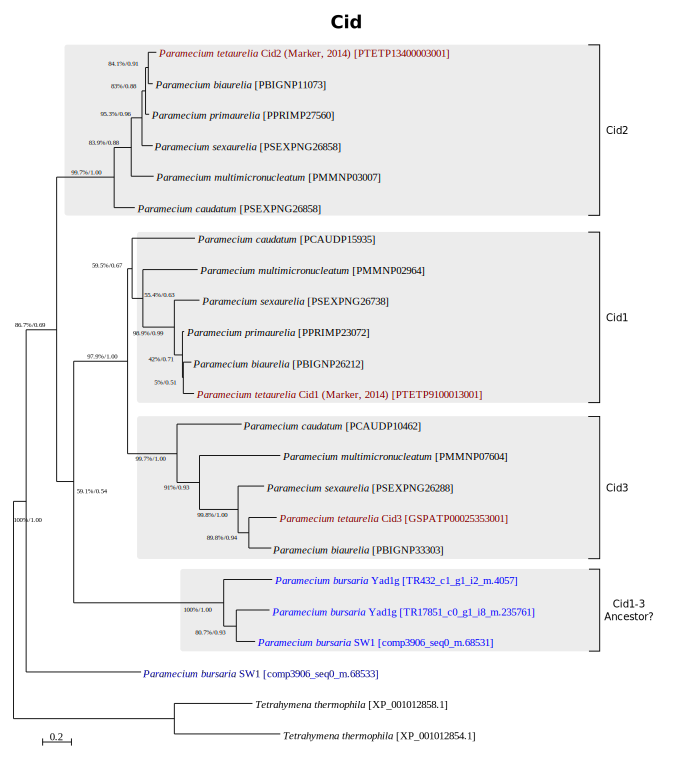
\includegraphics[width=\textwidth]{Cid.pdf}
    \caption[Phylogeny of Cid Sequences]{Bayesian
    and Likelihood phylogeny of CID components}
    \label{fig:cid_phlyo}
\end{figure}


\subsubsection{Rdr}


\begin{figure}
    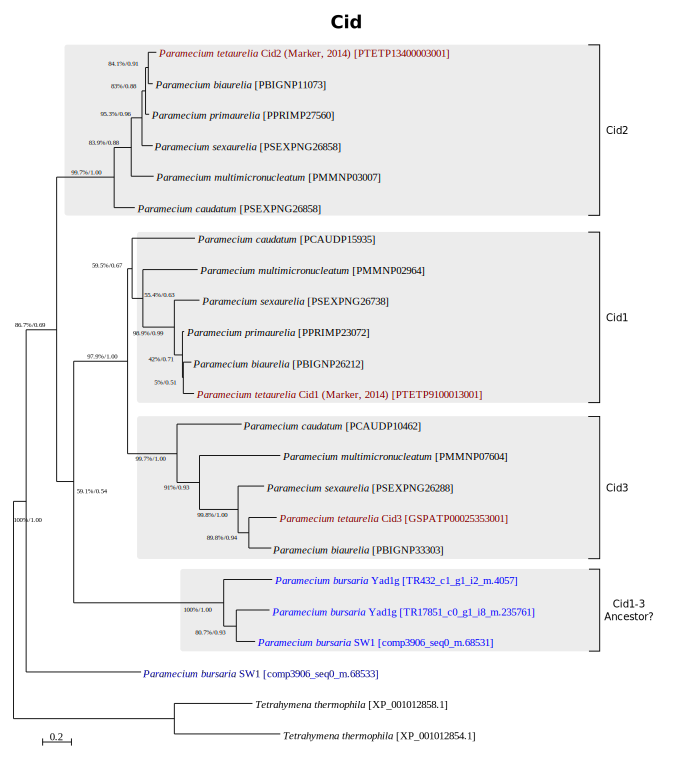
\includegraphics[width=\textwidth]{Cid.pdf}
    \caption[Phylogeny of Cid Sequences]{Bayesian
    and Likelihood phylogeny of CID components}
    \label{fig:cid_phlyo}
\end{figure}

\subsubsection{Piwi}



\subsection{RNAi cross-talk}

\begin{figure}
    \centering
    \includegraphics[width=\textwidth]{edicer_collisions.pdf}
    \caption[]{}
    \label{fig:edicer_collisions}
\end{figure}


\section{Discussion}

\subsection{Exogenous RNAi is non-functional in \textit{P. bursaria} CCAP 1660/12}

PSD1 is totally absent. 

Degenerate PCR was attempted using sequences from \textit{P. tetaurelia} and 
the other \textit{aurelia}


Feeding doesn't work 

Need to replicate using the \textit{P. bursaria} YADG1N strain

\subsection{Microinjection is methodologically difficult}

While RNAi by microinjection repeatedly failed there is a still a high possibility
that this is more related to the methodological difficulty of this technique rather than
necessarily any 
\cref{fig:microinjection_nucleus}

\begin{figure}
    \includegraphics[width=\textwidth]{microinjection_hard.pdf}
    \caption{}
    \label{fig:microinjection_nucleus}
\end{figure}


\subsection{Deactivation requires confirmation}





\subsection{Endosymbiont ``collision'' hypothesis}

Exogenous RNAi response is not essential for viability in \textit{P. tetaurelia}
\citep{Marker2014}.

However, the high degree of conservation even in \textit{P. bursaria}
suggests they play an important role. 

No \textit{Paramecium} viruses have been identified yet. 

Prseumably they exist, however it is possible that the endosymbiont plays a role.


\textit{C. elegans} has a dsRNA transporter (\textit{SID-2}) \citep{Nuez2012}


microinjection of fluore

often bursts after 1 injection, trichocysts block needle







Hypothetically, one explanation for the deactivation/loss
of RNAi in \textit{P. bursaria} CCAP 1660/12.




A regression analysis using a measure of phylogenetic distance would be interesting.
For example k-mer collisions by 100


Only finds exact matches though.




Finally, while this may not have thoroughly resolved the question of matches
eDicer may form a useful tool in the rapid screening of off-target effects
in the RNAi analyses in different organisms.   It is considerably
more efficient than exact matches 
than cut and alignment based methods. 





\section{Conclusions}

RNAi induced phenotypes could not be created in \textit{P. bursaria} CCAP1660/12
by either feeding experiments or direct transgene microinjection. 

Therefore, assembled transcriptomic and genomic data from \textit{P. bursaria}
CCAP 1660/12 and YADG1N were analysed for factors identified as essential in the function
of these pathways in \textit{P. tetaurelia} \citep{Marker2014}. 

\begin{figure}
    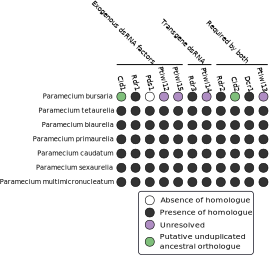
\includegraphics[width=\textwidth]{RNAi_factors_summary_figure.pdf}
    \caption[Summary of RNAi Factors Presence]{Summary of the discovery
    of RNAi figures in \textit{P. bursaria}}
    \label{fig:rnai_summary}
\end{figure}

Two proteins essential for the function of the exogenous dsRNA induced
RNAi pathway in \textit{P. tetaurelia}, Pds1 and Rdr1, were not found in the partial genome and transcriptome 
of \textit{P. bursaria} CCAP 1660/12 or the transcriptome of \textit{P. bursaria} YADG1N.
This suggests that this pathway may not be active/present in \textit{P. bursaria}.
Either, 


However, assuming the likely pre-duplication orthologue of Cid2 and the necessary 
unresolved Ptiwi's are functional
in the transgene dsRNA pathway of \textit{P. bursaria}
then this pathway is theoretically active.  Unfortunately, methodological
difficulties in microinjection have thus far failed to generate RNAi-induced
phenotypes.
